\documentclass{article}
\usepackage[a4paper, margin={1in, 1in}]{geometry}
\usepackage[utf8]{inputenc}
\usepackage{polski}
\usepackage{mathtools}
\usepackage{amsfonts}
\usepackage{amssymb}
\usepackage{amsmath}
\usepackage{multicol}
\usepackage{paralist}
\usepackage{tabto}
\usepackage{graphicx}
\usepackage{etoolbox}
\usepackage{changepage}
\usepackage{tasks}
\usepackage{pgfplots}
\usepackage{fancyhdr}

\DeclareMathOperator{\arctg}{arctg}
\DeclareMathOperator{\sh}{sh}
\DeclareMathOperator{\ch}{ch}
\DeclareMathOperator{\sgn}{sgn}

\let\arctan\relax
\DeclareMathOperator{\arctan}{arctg}
\let\tan\relax
\DeclareMathOperator{\tan}{tg}

% Dodatkowe deklaracje:

\usepackage{subcaption}

\usetikzlibrary{patterns}
\usetikzlibrary{intersections}
\usepgfplotslibrary{fillbetween}

\newcommand{\Because}{\quad\because\quad}
\newcommand{\case}[1]{\textrm{#1$^\circ$}}
\newcommand{\degree}{^{\circ}}
\newcommand{\diff}{\mathop{}\!\mathrm{d}}
\newcommand{\for}{\ \leftrightarrow\ }
\newcommand{\Integral}[4]{\int_{#1}^{#2} \! #3 \, \mathop{}\!\mathrm{d}#4}
\newcommand{\mathcolorbox}[2]{\colorbox{#1}{$\displaystyle #2$}}
\newcommand{\norm}[1]{\left\lVert#1\right\rVert}
\newcommand{\qed}{\textbf{\textit{QED}}}
\newcommand{\qef}{\textbf{\textit{QEF}}}
\newcommand{\task}[1]{\textit{#1}}
\newcommand{\xrowht}[2][0]{\addstackgap[.5\dimexpr#2\relax]{\vphantom{#1}}}
\newcommand{\partderiv}[2]{\frac{\partial #1}{\partial #2}}

\DeclareMathOperator{\?}{?}
\DeclareMathOperator{\dom}{dom}
\DeclareMathOperator{\im}{im}
\DeclareMathOperator{\lin}{lin}
\DeclareMathOperator{\N}{\mathbb{N}}
\DeclareMathOperator{\R}{\mathbb{R}}
\DeclareMathOperator{\Z}{\mathbb{Z}}

\let\oldepsilon\epsilon \renewcommand{\epsilon}{\varepsilon}

% Koniec dodatkowych deklaracji

\pagestyle{fancy}

\lhead{Analiza Matematyczna 2; 2020/2021}
% Tutaj proszę uzupełnić imię i nazwisko
\rhead{Jakub Łukasiewicz}

\begin{document}
\section*{Zadanie 1a}

Zmienić kolejność całkowania w całce iterowanej
$ \displaystyle \Integral{-1}{1}{}{x} \Integral{0}{|x|}{f(x,y)}{y} $

\subsection*{Rozwiązanie}

Z całki wynika, że obszar całkowania $D$ jest ograniczony poprzez:
\quad $ -1 \le x \le 1,\quad 0 \le y \le |x| $

\begin{figure}[h!]
   \centering
   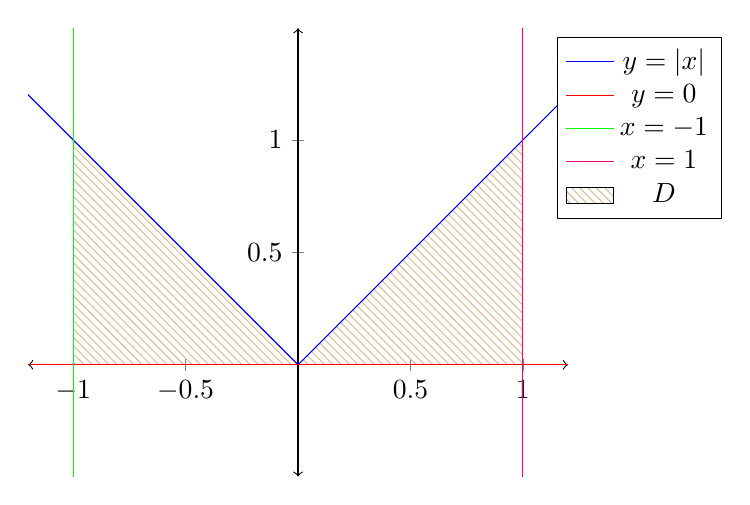
\begin{tikzpicture}
      \begin{axis}[
            xmin=-1,xmax=1,
            ymin=0,ymax=1,
            axis lines=middle,
            axis line style=<->,
            axis equal,
            enlargelimits,
            domain=-2:2,
            samples=3,
            legend style={anchor=north west}]
         ]
         \addplot[name path=F, blue] {abs(x)};
         \addplot[name path=G, red] {0};

         \addplot +[mark=none, green] coordinates {(-1, -1) (-1, 2)};
         \addplot +[mark=none, magenta] coordinates {( 1, -1) ( 1, 2)};

         \addplot[pattern=north west lines, pattern color=brown!50]fill between[of=F and G,  soft clip={domain=-1:1}];

         \legend{$y=|x|$, $y=0$, $x=-1$, $x=1$, $D$}
      \end{axis}
   \end{tikzpicture}
\end{figure}

Zatem maksymalna wartość jaką przyjmuje $y$ to $1$, stąd $0 \le y \le 1$.

Teraz obszar dzielimy na dwa obszary wg osi $0y$: "ujemny" $D_1$ i "dodatni" $D_2$

\begin{figure}[h!]
   \centering
   \begin{subfigure}[b]{0.4\textwidth}
      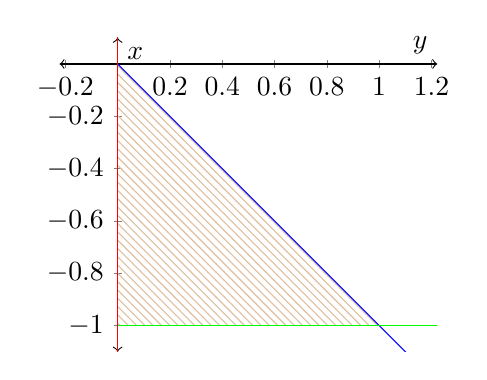
\begin{tikzpicture}[scale=0.7]
         \begin{axis}[
               xmin=0,xmax=1,
               ymin=-1,ymax=0,
               axis x line=middle,
               axis y line=middle,
               axis line style=<->,
               xlabel={$y$},
               ylabel={$x$},
               axis equal,
               enlargelimits,
               domain=0:2,
               samples=3,
            ]
            \addplot[name path=F, blue] {-abs(x)};
            \addplot[name path=G, green] {-1};
            \addplot[mark=none, red] coordinates {(0, -2) (0, 2)};
            \addplot[pattern=north west lines, pattern color=brown!50]fill between[of=F and G,  soft clip={domain=-1:1}];
         \end{axis}
      \end{tikzpicture}
   \end{subfigure}
   %
   \begin{subfigure}[b]{0.4\textwidth}
      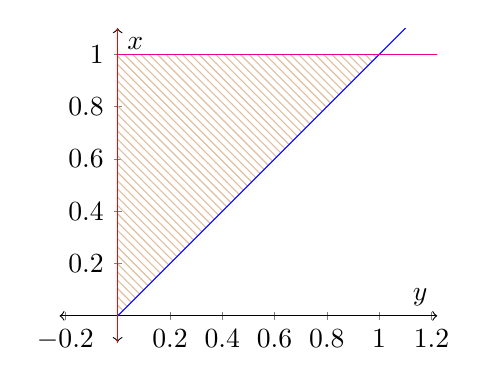
\begin{tikzpicture}[scale=0.7]
         \begin{axis}[
               xmin=0,xmax=1,
               ymin=0,ymax=1,
               axis x line=middle,
               axis y line=middle,
               axis line style=<->,
               axis equal,
               xlabel={$y$},
               ylabel={$x$},
               enlargelimits,
               domain=0:2,
               samples=3,
            ]
            \addplot[name path=F, blue] {abs(x)};
            \addplot[name path=G, magenta] {1};
            \addplot[mark=none, red] coordinates {(0, -2) (0, 2)};
            \addplot[pattern=north west lines, pattern color=brown!50]fill between[of=F and G,  soft clip={domain=-1:1}];
         \end{axis}
      \end{tikzpicture}
   \end{subfigure}
\end{figure}

Z wykresów odczytujemy, że w obszarze
\begin{itemize}
   \item $D_1$ mamy $x = -y,\ y\le 1$, zatem $-1 \le x \le -y$.
   \item $D_2$ mamy $x = y,\ y \le 1$, zatem $y \le x \le 1$.
\end{itemize}

Stąd możemy podać odpowiedź.

\subsection*{Odpowiedź}

\begin{equation*}
   \Integral{0}{1}{}{y} \Integral{-1}{-y}{f(x,y)}{x}
   \ +\
   \Integral{0}{1}{}{y} \Integral{y}{1}{f(x,y)}{x}
\end{equation*}

\end{document}
